\documentclass[a4paper,12pt]{article}

% --- Packages ---
\usepackage[utf8]{inputenc}
\usepackage[T1]{fontenc}
\usepackage[english]{babel}
\usepackage{graphicx}
\usepackage{amsmath, amssymb}
\usepackage{hyperref}
\usepackage{natbib}
\usepackage{geometry}
\geometry{margin=2.5cm}

% --- Title Info ---
\title{Praktikum Data Science: Phase 1 Report}
\author{Éva Mária Szabó \\ \small Karlsruher Institut für Technologie (KIT)}
\date{\today}

\begin{document}

% --- Title Page ---
\maketitle
\tableofcontents
\newpage

% --- Sections ---
\section{Introduction}
In my team, which is Team 3, we did most parts fo our excercise in a pair programming style. Due to that most commits are not under my name, since I was not the one who pushed them. However, I still contributed a lot of work to the project, so I will summarize my contributions here.

\section{Week 1 - Data Exploration}
To kick things off, I did some bar charts and pie charts regarding the data. 
\begin{figure}
    \centering
    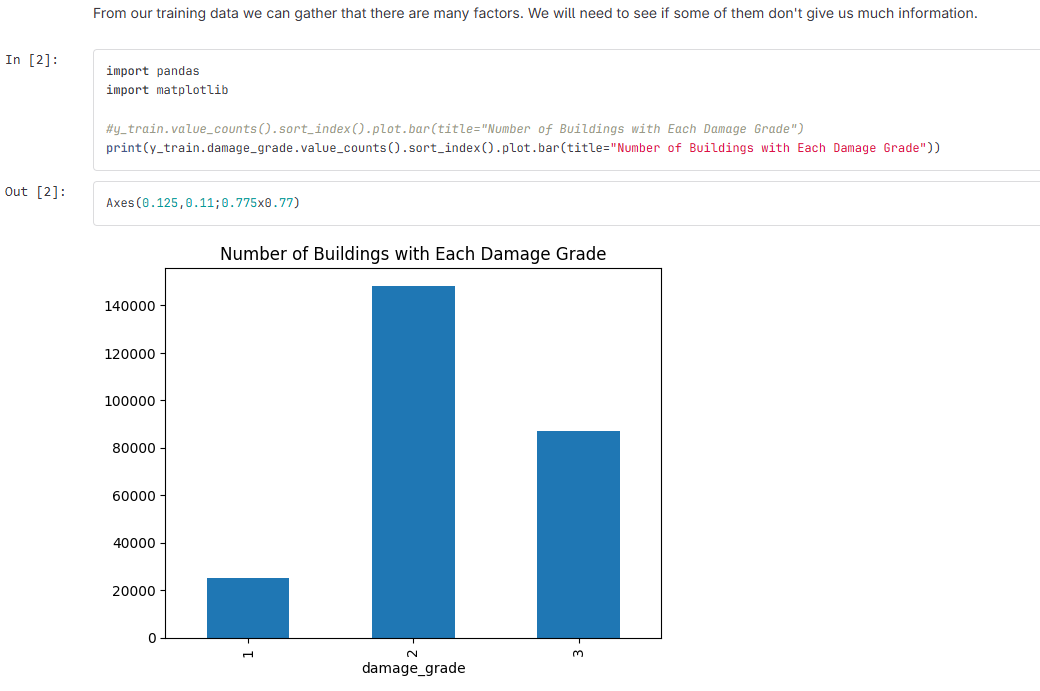
\includegraphics[width=0.8\textwidth]{figures/example_plot_jupyter.png}
    \caption{Example of a plot I created in Jupyter Notebook}
    \label{fig:data_exploration}
\end{figure}
In Figure~\ref{fig:data_exploration}, you can see an example of a plot I created in Jupyter Notebook. This helped us to understand the data better and identify potential issues.
I also wrote some initial code to load the data and perform basic statistics, which was crucial for our understanding of the dataset, as well as commenting each plot and what conclusions we drew from them.

\section{Week 2 - Cleaning and pipeline}
From this week onwards I was responsible for researching. For this week this meant looking into how to clean the data and how to set up a pipeline for our data processing. I found out that we can use the \texttt{sklearn} library for this purpose, which is very powerful and flexible. I also wrote some initial code to clean the data and a pipeline structure, which was crucial for our understanding of the dataset. Since I had previously worked on some data science projects, I was able to apply my knowledge and experience to this project, such as how to treat missing values, how to encode categorical variables, and how to scale numerical features.

\section{Week 3 - Feature Engineering}
We've had much discussions about which features to use and how to create new ones. I researched various feature engineering techniques, dolgok dolgok

\section{Week 4 - Prediction Models}
Since we discussed that I will be holding the presentation for this week, I focused on understanding different prediction models. I researched various algorithms such as logistic regression, decision trees, and random forests. I also implemented some of these models in Python using the \texttt{sklearn} library. This helped us to understand the strengths and weaknesses of each model and how to choose the best one for our dataset. I also wrote some initial code to evaluate the models and compare their performance, which was crucial for our understanding of the dataset.

\section{Week 5 - Dealing with Imbalanced Multi-Class Data}
Tried to do a threshold tuning but that did not work out as expected. I researched various techniques to deal with imbalanced multi-class data, such as oversampling, undersampling, and using different evaluation metrics. I also implemented some of these techniques in Python using the \texttt{sklearn} library. This helped us to understand how to handle imbalanced data and how to choose the best evaluation metric for our dataset. I also wrote some initial code to evaluate the models and compare their performance, which was crucial for our understanding of the dataset.

\section{Week 6 - Hyperparameter Tuning}
For this week it was Ádám's turn to present, so he did most of the work. However, I continued my research on cross-validation and different prediction models. I also helped him to prepare the presentation and provided some feedback on his slides. That means I did all of the plots for it. 

\section{Conclusion}
In conclusion, I contributed significantly to the project by researching various topics, implementing code, and preparing presentations. I learned a lot about data science and how to apply it to real-world problems. I also enjoyed working in a team and collaborating with my teammates. I hope that my contributions will help us to achieve our goals and complete the project successfully.

% --- Bibliography ---
%\bibliographystyle{plainnat}
%\bibliography{mybib}

\end{document}
